\documentclass{article}

\usepackage{graphicx}
\usepackage[ngerman]{babel}
\usepackage{datetime}
\usepackage{float}

\title{Projektarbeit \\ Datenbankding}
\date{08-06-2021}
\author{Severin Gafner \and David Hänni}
\newdateformat{germanformat}{\THEDAY{ }\monthname[\THEMONTH], \THEYEAR}
\def\Cmodule{Objektorientiertes Programmieren 2} 
\def\Ctitle{DatationBase} 
\def\Cauthor{Severin Gafner | David Hänni} 
\def\Cschool{TEKO Schweizerische Fachschule} 
\begin{document}

\begin{titlepage}
	\centering
	
\includegraphics[width=0.3\textwidth]{images/teko-logo-pink.jpg}\par\vspace{1cm}
	{\scshape\LARGE \Cschool\par}
	\vspace{1cm}
	{\scshape\Large Semesterarbeit \\ \Cmodule\par}
	\vspace{1.5cm}
	{\huge\bfseries \Ctitle\par}
	\vspace{2cm}
	{\Large\itshape \Cauthor\par}
	\vfill
	begleitet durch\par
	Herr Christian \textsc{Herren}

	\vfill

	{\large \germanformat\today\par}
\end{titlepage}
\pagenumbering{gobble}
\newpage
\pagenumbering{arabic}

\section{Einleitung}

Severin Gafner und David Hänni führen im Rahmen des Studiums zum Techniker HF Applikationsentwicklung für das Modul \Cmodule eine Semesterarbeit durch. 

\section{Aufgabenstellung}
Nachfolgend die Umschreibung der Aufgabenstellen 1:1 aus dem Auftrag kopiert.
\subsection{Umschreibung der Aufgabenstellung}
Wir sind die IT-Firma NewIdeas und wir haben die nachfolgende Geschäftsidee: 
Im Zusammenhang mit Automationsvorhaben werden von unseren Kunden immer mehr kleine aber individuelle Lösungen gesucht. 
Wir haben nun festgestellt, dass sich die bekannten (umfangreichen) Datenbanksysteme für derartige Vorhaben nicht oder nur bedingt eignen, vor allem die teilweise abstrus teuren Lizenzmodelle lassen diese als nur bedingt tauglich erscheinen. 
Die verfügbaren OpenSource/Freewarelösungen können wir nicht ernst nehmen resp. wollen wir aus Gründen der Nachhaltigkeit nicht verwenden.
\section{Projektumfeldanalyse}
Mit der Projekumfeldanalyse werden möglichst viele Information über vorhandene Interessen, Bedürfnisse, Einflussmöglichkeiten und Beziehungen im Projektumfeld ermittelt.
\subsection{Stakeholder}
\begin{figure}[H]
	\centering
  	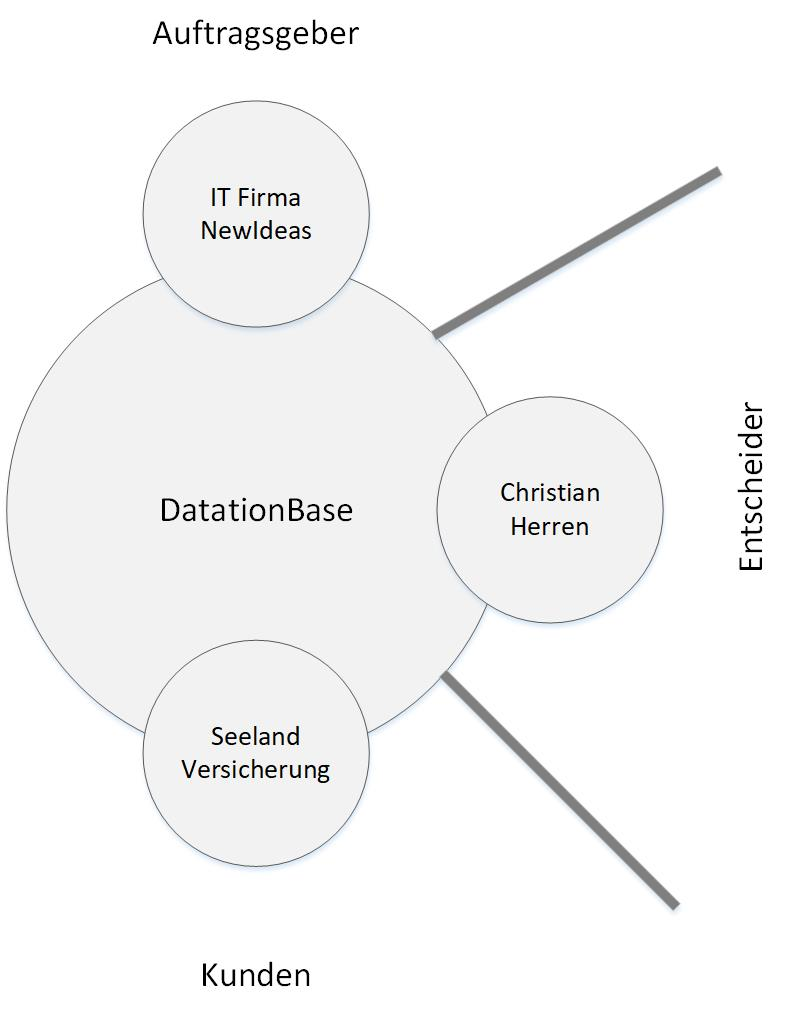
\includegraphics[width=0.7\linewidth]{images/stakeholder.jpg}
  	\caption{Identifizierte Stakeholder}
 	\label{fig:stakeholder}
\end{figure}
Die Stakeholder wurden in drei Kategorien eingeteilt:
\paragraph{Auftraggeber}
Der Auftraggeber ist die IT Firma NewIdeas. Ihr Ziel ist es, ihre Kunden mit einer eigenen Datenbanklösung an sich zu binden und so zukünftige Wartungen und Modifikationen an der Lösung durchführen zu können.
\paragraph{Kunden}
Als erstes Kunde wird die Seeland-Versicherung die Datenbank einsetzen. Später werden weitere Kunden dazustossen. Der Kunde möchte eine performante Datenbank ohne Datenverlust.
\paragraph{Entscheider}
Christoph Herren ist ebenfalls ein Stakeholder dieses Projektes. Er überwacht die Durchführung der Arbeit und bewertet das Endresultat.
\subsection{Situationsanalyse Seeland-Versicherung}
Die Seeland-Versicherung spielt als erster Kunde eine sehr wichtige Rolle. Mit den 1'500 Kunden und 450 Schadensfälle pro Jahr beinhaltet die Datenbank nur wenig Datensätze. Angenommen es werden die Schadensfälle der letzten 20 Jahre migriert, so umfasst die Datenbank immer noch nur knapp 10'000 Datensätze.
\section{Ziele}
Die Projektziele zeigen auf, was erreicht werden muss.
\subsection{MUSS-Ziele}
\subsubsection{Anforderungen geklärt}
Die funktionalen und nicht-funktionalen Anforderungen an das Produkt sind klar definiert.
\subsubsection{Use-Cases definiert}
Use Cases wurden nach UML Richtlinien definiert und beschrieben.
\subsubsection{Testkonzept erstellt}
Ein Testkonzept wurde erstellt, welches die Testmethoden, die hilfmittel und die Testanlagen beschreiben. Zu jedem Use Case wurde mindestens ein positiv und ein negativ Test erfasst.
\subsubsection{Systemarchitektur beschrieben}
Die Systemarchitektur und die einzelnen Komponenten sowie deren Schnittstellen wurden beschrieben.
\subsubsection{Fertigstellung erreicht}
Das Produkt ist einsatzfähig und hat alle Testszenarien vom Testkonzept bestanden. Alle Use Cases wurden implementiert.
\subsection{KANN-Ziele}
\subsubsection{Datenimport}
Über eine Schnittstelle können aus einer Datei direkt in die Datenbank importiert werden.
\section{Anforderungen}
Die Anforderungen an das Produkt werden von den Zielen Abgeleitet. Sie werden in funktionale und nicht-funktionale Anforderungen aufgeteilt.
\subsection{Funktionale Anforderungen}
\subsubsection{Tabellen definierten}
Es können Tabellen mit unterschiedlichen Namen definiert werden.
\subsubsection{Felder definieren}
Auf einer Tabelle können Felder erfasst werden. Diese Felder besitzen einen Namen und einen der folgenden Datentypen: string, int, boolean
\subsubsection{Datensätze hinzufügen}
Auf einer bestehenden Tabelle können über eine C\# Methode mehrere neue Datensätze hinzugefügt werden.
\subsubsection{Datensätze löschen}
Auf einer bestehenden Tabelle kann über eine C\# Methode mehrere bestehender Datensätze gelöscht werden.
\subsubsection{Datensätze verändert}
Auf einer bestehenden Tabelle kann über eine C\# Methode mehrere bestehender Datensätze verändert werden.
\subsubsection{Datensätze anzeigen}
Auf einer bestehenden Tabelle kann über eine C\# Methode mehrere bestehender Datensätze ausgelesen werden.
\subsubsection{Schnittstelle XML}
Über eine Schnittstelle können Daten im XML Format in die Datenbank importiert werden.
\subsubsection{Schnittstelle JSON}
Über eine Schnittstelle können Daten im JSON Format in die Datenbank importiert werden.
\subsubsection{Schnittstelle CSV}
Über eine Schnittstelle können Daten im CSV Format in die Datenbank importiert werden.
\subsubsection{}
\subsection{Nicht funktionale Anforderungen}
\subsubsection{Speichervolumen}
Das Produkt muss mindestens eine 2GB grosse Datenbank mit 1'000'000 Datensätzen bewältigen können.
\subsubsection{Zugriffszeiten}
Bei 100'000 Datensätzen darf die Zugriffszeit auf einen Datensatz nicht länger als 100 ms dauern.
\subsubsection{Programmiersprache}
Die Datenbank wird mittels C\# implementiert.
\subsubsection{Projektabgabe}
Das Produkt sowie die Projektdokumentation müssen bis am 28.09.2021 um 18:30 Uhr abgegeben sein.


\end{document}